\documentclass[12pt]{article}

\input preamble

\title{Principles of Parallel Architecture\\
Homework 1: Parallel Benchmarks}
\author{Xitong Liu \\
xliu@ece.udel.edu}

\begin{document}

\maketitle

\section{Question 1}
[35\%] The TOP 500 is a widely recognized organization that lists the 500 
supercomputers with the most performance in terms of absolute computational 
rate and computational efficiency. Please visit the TOP 500 website: 
\texttt{http://www.top500.org/} and navigate through the site to learn about 
TOP 500.

\begin{enumerate}

\item
\begin{description}
\item[Q: ]According to what the performance is measured? How often the 
rank is updated?
\item[A:]The performance is measured by their performance on the LINPACK 
Benchmark. The rank is updated twice a year.
\end{description}

\item
\begin{description}
\item[Q: ]Plot the performance of the fastest supercomputer vs time since 
1993. What can you comment on this plot?
\item[A: ]According to Fig.\ref{fig:fatest}, 
\begin{figure}[h!]
	\begin{center}
		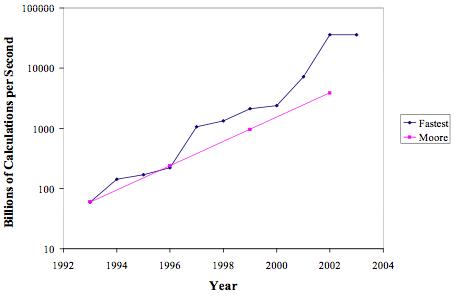
\includegraphics[width=0.7\textwidth, angle=0]{fatest.png}
		\caption{\label{fig:fatest}Fatest SuperComputer in the world}
	\end{center}
\end{figure}
the computing speed doubled roughly every 18 months, following 
the \textbf{Moore's Law}.
\end{description}

\item
\begin{description}
\item[Q: ]Using the statistics tool, generate plots for Architecture, 
Processor Architecture, Processor Family and Number of Processors over 
time. Make conclusions about the progress in these characteristics. 
Where are going the supercomputers according to these characteristics? 
Explain briefly.
\item[A: ]Plots listed as below:
\begin{figure}[h!]
	\begin{center}
		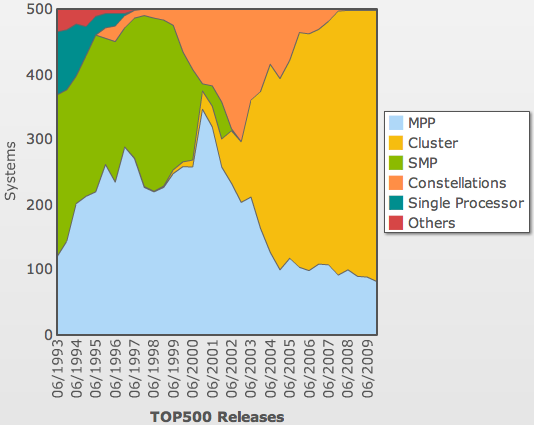
\includegraphics[width=0.7\textwidth, angle=0]{arch-share.png}
		\caption{\label{fig:arch-share}Architecture Share Over Time 1993-2009}
	\end{center}
\end{figure}
\begin{figure}[h!]
	\begin{center}
		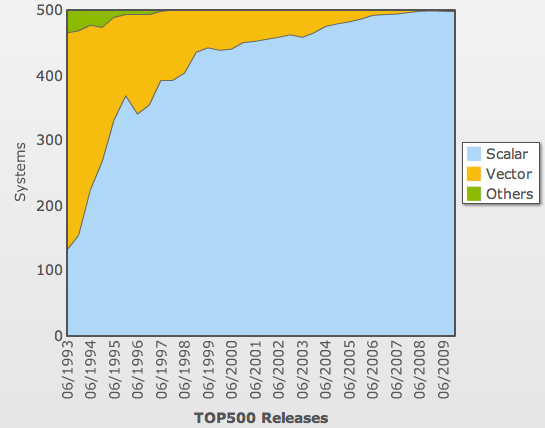
\includegraphics[width=0.7\textwidth, angle=0]{proc-arch-share.png}
		\caption{\label{fig:proc-arch-share}Processor Architecture Share Over Time 1993-2009}
	\end{center}
\end{figure}
\begin{figure}[h!]
	\begin{center}
		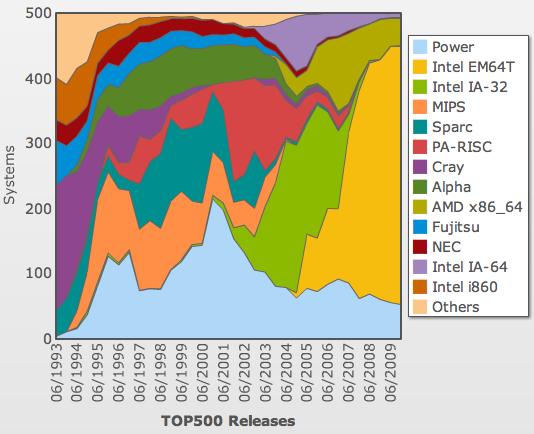
\includegraphics[width=0.7\textwidth, angle=0]{proc-family-share.png}
		\caption{\label{fig:proc-arch-share}Processor Family Share Over Time 1993-2009}
	\end{center}
\end{figure}
\begin{figure}[h!]
	\begin{center}
		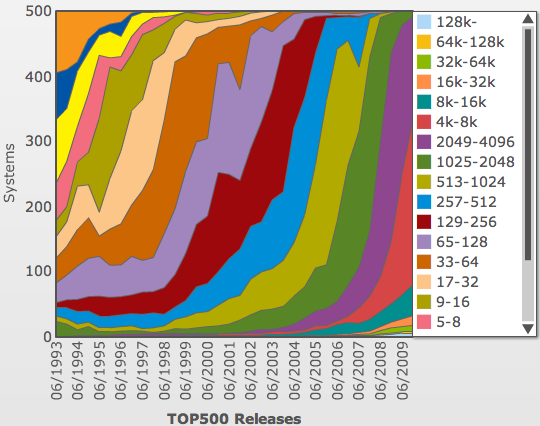
\includegraphics[width=0.7\textwidth, angle=0]{proc-num-share.png}
		\caption{\label{fig:proc-num-share}Number of Processors Share Over Time 1993-2009}
	\end{center}
\end{figure}
As the development of Super Computers, Cluster began to dominate the architecture, 
and most of the processors were scaler based. What's more, Intel EM64T began to 
dominate the processor market in the recent years. The number of processors of one 
super computer bumped dramatically 
in the recent years.
\end{description}

The Green500 provides rankings of the most energy-efficient supercomputers in the 
world. They raise awareness about power consumption, promote alternative total 
cost of ownership performance metrics, and ensure that supercomputers only simulate 
climate change and not create it. Please visit the green 500 website: 
\texttt{http://www.green500.org/}

\item
\begin{description}
\item[Q: ]Plot the computational rate per watt vs time for the top 5 supercomputer 
according to the MFLOPS/W since November 2007. Are they in the top 5 according 
performance? Comment on the evolution of power efficiency of supercomputers.
\item[A: ] See plot
\begin{figure}[h!]
	\begin{center}
		\includegraphics[width=\textwidth, angle=0]{green-top5.pdf}
		\caption{\label{fig:green-top5}Computational Rate Per Watt Over Time 2007-2009}
	\end{center}
\end{figure}
They are not the top5 according to performance. As the development of super computer,
it's more and more energy efficient.

\end{description}


\end{enumerate}

\end{document}